\documentclass{amsart}
\usepackage{graphicx}% Include figure files

\newtheorem{theorem}{Theorem}[section]
\newtheorem{lemma}[theorem]{Lemma}

\theoremstyle{definition}
\newtheorem{definition}[theorem]{Definition}
\newtheorem{example}[theorem]{Example}
\newtheorem{xca}[theorem]{Exercise}

\theoremstyle{remark}
\newtheorem{remark}[theorem]{Remark}

\numberwithin{equation}{section}

\begin{document}

\title{The accuracy of physics}

%    Remove any unused author tags.

%    author one information
\author{Peifeng Wang}
\address{Guanghua Road 1\#, 34-1-3-5, Yanta District, Xi'an, Shaanxi, P. R. China 710075}
\curraddr{}
\email{peifeng\_w@yahoo.com}
\thanks{Guanghua Road 1\#, 34-1-3-5, Yanta District, Xi'an, Shaanxi, P. R. China 710075}
\thanks{peifeng\_w@yahoo.com}

%    author two information
%\author{}
%\address{}
%\curraddr{}
%\email{}
%\thanks{}

%\subjclass[2010]{Primary }

\keywords{}

\date{}

\dedicatory{}

\begin{abstract}
Physics theories modeling physics realities are studied within the framework of set theory. It is shown that, only countable sets can be explicitly expressed in theory. If a physics reality comprises uncountable set, physics theories will not be able to accurately represent the reality to the full extent.
\end{abstract}

\maketitle

Physics theories are developed to model physics realities, from the farthest stars in outer space to the tiniest particles inside nuclei. One common expectation is that the theories can accurately describe the realities. Although accuracy may seem relevant mainly in dealing with experiments, it is also inherent in a pure theoretical context. A valid question is, what is the accuracy of physics theories and realities? Or alternatively, can physics theories model physics realities in complete accuracy?

Informally, since it is impossible to accurately write down an irrational number, physics theories can not describe physics realities in full accuracy. As any deficiency in accuracy will leave a prediction deviate from reality, physical world can be deterministic while unpredictable.

For a detailed discussion, a metamodel of physics theories is presented, elements of physics theories are examined within set theory. With rational number and real number being instances of countable set and uncountable set respectively, it is shown that, a theory can only explicitly express a countable set, but physics reality comprises uncountable sets, thus physics theories will not be able to accurately represent the reality to the full extent.

In a metamodel similar to mathematic logic\cite{Zaring,Sheppard}, physics theories consist of the following 4 types of elements

1) Constants include mathematics constants (e.g. $\pi$, $\sqrt{2}$) and physics constants (e.g. speed of light c, Plank constant h, ...)

2) Variables are quantities associated with physical properties (e.g. length L, time t, velocity $\mathbf v$, current density $\mathbf J$, ...)

3) Formulas are groups of symbols of constants and variables joined in certain patterns (e.g. $E=mc^2$, Maxwell equations, $\mathbf a=\dot{\mathbf v}$, ...)

4) Inference rules comprise mathematics theorems (e.g. arithmetics, calculus, algebras, logics)

Each element plays a role in the metamodel. Both constants and variables are quantities. While constants remain unchanged in physical world, variables represent varying states of physics reality. Formulas describe physics mechanism by defining relations between physics quantities (constants and variables). Inference rules are tools to transform variables and formulas into various formats for analysis.

In the study of physics to model reality with theory, maps between reality and theory are defined in the form of variables and formulas. As a typical example, the definition of length/distance, a key element of geometric coordinates which is fundamental for many analyses, is examined. In reality, the original aim was to differentiate the states of extremely short, much shorter, somehow shorter, slightly shorter, slightly longer, somehow longer, much longer, extremely long and others in between and/or outside the listed ones. For this purpose, a length in reality is mapped into a number in theory, and a variable L is introduced in theory.

The variable L bears multiple meanings. It appears a number in theory, and it refers to a length in reality. It is also the translation between the length in reality and the number in theory, which, in practices,  involves experimental measurements. In an ideal situation, a length in reality can be identified by a number in theory and two lengths in reality can be compared by comparison of their corresponding numbers in theory.

More generally, a physics variable designates a mapping between certain states in reality and entities in theory. Specifically, there is a set $\mathbb{S}$ of states in reality and a set $\mathbb{E}$ of entities in theory, then a variable V is a mapping $V: \mathbb{S}\leftrightarrow \mathbb{E}$. The set $\mathbb{E}$ is a theoretical representation of reality $\mathbb{S}$, and the set $\mathbb{S}$ is the underlying reality of theoretical entities $\mathbb{E}$. The map is bidirectional so that in the case of experimental measurement, states in reality are mapped into entities in theory, while in the case of theoretical description, entities in theory are mapped into states in reality.

To faithfully represent reality with theory, an ideal mapping of a variable is supposed to be bijective and order preserving. However, as the choice of set $\mathbb{E}$ is subject to various factors, it is not always in bijection with the set $\mathbb{S}$ in reality. Thus $\mathbb{E}$ may be only an approximation of reality $\mathbb{S}$.

Then the accuracy of a variable depends on the choice of set $\mathbb{E}$. Normally, the set $\mathbb{E}$ of entities in theory is a set of numbers, then the mapping of a variable is just the familiar process of quantization in measurements. e.g. let $\mathbb{N}$ be the set of natural numbers, if $\mathbb{E}=\{0.1i|i\in\mathbb{N}\}$ is a set of multiples of 0.1, then the variable V is modeled by the set of numbers \{0.1, 0.2, ..., 1.0, 1.1, ...\}, and its accuracy is 0.1.

Empirically, the choice of set $\mathbb{E}$ is constrained by the capacity of measurement apparatus, which is well studied. But completely independent of considerations of experimental measurement, there is a purely theoretical restriction on achievable accuracy.

The theoretical limit of achievable accuracy is due to the expressiveness of theories. To clarify, the definition of accuracy can be generalized. An element is at first order accuracy if it is modeled by a countable set. An element is at second order accuracy if it is modeled by an uncountable set.

As to be shown, the set $\mathbb{E}$ of entities in theory and the set $\mathbb{S}$ of states in reality are having different cardinalities. Thus the mapping $V: \mathbb{S}\leftrightarrow \mathbb{E}$ can not be bijective, and the theoretical $\mathbb{E}$ can not exactly represent reality $\mathbb{S}$.

The study of physics serves the purpose of understanding the world explicitly and accurately. Explicitness ensures that a result is in a concrete form, while accurateness guarantees that a result reveals reality. An understanding is deficient if it is not both explicit and accurate.

To be explicit, every entity in a theory is expressed in a finite form, i.e. a finite sequence of symbols. Even a concept of infinity is represented finitely. e.g. the string ``1, 1.4, 1.41,1.414, 1.4142, ..." is an entity referring to an infinite sequence converging to $\sqrt 2$, yet the string is finite and the meaning of infinity is conveyed by the finite symbol ``...". The expression size of an entity is defined to be the number of symbols that are used to express that entity.

Let $\mathbb{A}$ be the set of all entities that can be explicitly expressed, i.e. every element $e\in\mathbb{A}$ can be explicitly expressed and has finite expression size. Then elements of $\mathbb{A}$ can be enumerated in the following order: first list all elements of expression size 1, then list all elements of expression size 2, then list all elements of expression size 3, ... Therefore $\mathbb{A}$ is a countable set. As elements of $\mathbb{E}$ are required to be explicitly expressed, $\mathbb{E}\subset\mathbb{A}$ is also countable.

Conversely, for an uncountable set $\mathbb{\bar A}$, there exist elements $e\in\mathbb{\bar A}$ with infinite expression size. i.e. some elements of an uncountable set have infinite expression size, thus can not be explicitly expressed.

Therefore, certain mathematical entities are not explicitly and accurately expressed. In specific, the set of irrational number is uncountable, it is impossible to accurately express an irrational number in its completeness. In a theoretical context, an irrational number has infinite expression size, so that it only reveals its various aspects but not its entirety.

For example, $\pi$ refers to an entity, which, in the simplest sense, is a number. Alternatively, it is the ratio between the circumference and diameter of a circle, it is half of the period of sinusoidal function, it is also a never ending algorithm that takes months for a computer to calculate trillions of digit, or it is the limit of sequence: 3, 3.1, 3.14, 3.141, 3.1415, ... It is understood that a certain entity bears all these properties, but that entity can not be written down in its full form. The symbol $\pi$ is used to designate that entity without bothering all of its digits.

While tokens are assigned to certain irrational numbers, e.g. $\pi,\sqrt 2$, not every irrational number can have a token. Since every token must be explicitly expressed, the set of all tokens is a subset of $\mathbb{A}$, thus countable. But the set of irrational number is uncountable. Therefore, there are not enough many tokens to be distinctively assigned to each irrational number. Thus, the majority of irrational number can neither be explicitly expressed, nor be represented by a token. These irrational numbers are unexplored in theoretical context.

Unlike irrational number, the set of rational number is countable, and any rational number can be fully represented as a ratio between two integers. As a result, physics theories express conclusions with rational numbers. Where an irrational number is qualitatively needed, physics theories use a token to refer to that irrational number. When quantitative analysis is required, physics theories use a rational number to approximate an irrational number.

\begin{figure}
\center
\fbox{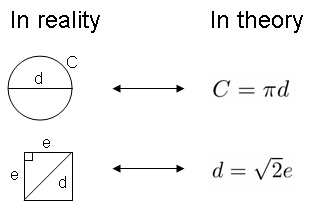
\includegraphics{irrational.png}}
\caption{Irrational numbers arise in reality and are represented by tokens in theory}
\label{fig:irrational}
\end{figure}
On the other hand, irrational numbers attain their full accuracy in physics reality. For examples in fig. \ref{fig:irrational}, a circle exists in reality, both its circumference and diameter are lengths in reality. The ratio of the circumference to the diameter exists accurately in reality, and that ratio is an irrational number, designated by $\pi$. Likewise, a square exists in reality, its edge e and diagonal d are both lengths in reality. The ratio of diagonal to edge exists accurately in reality, which is an irrational number, designated by $\sqrt 2$.

In addition, the real line exists in reality. Every point on the real line corresponds to a real number, and every pair of points on the real line gives rise to a length in reality. Then the set of all lengths in reality is uncountable. Therefore, the set of states in reality is uncountable, i.e. $\mathbb{S}$ is uncountable.

It follows that, while the set $\mathbb{E}$ of entities in theory is countable, the set $\mathbb{S}$ of states in reality is uncountable. As a result, the mapping of a variable $V: \mathbb{S}\leftrightarrow \mathbb{E}$ is not bijective, instead, it resembles a statistical experiment, in which a subset of a population is sampled to represent the population. Variable V models the uncountable set $\mathbb{S}$ of states in reality with a countable set $\mathbb{E}$, consequently it can only approximately, but not exactly represent reality $\mathbb{S}$ with the theoretical $\mathbb{E}$.

In physics, multiple variables may be interdependent, their relations are revealed by formulas. By symbolization of constants and variables, formulas can be presented in an explicit form without being concerned with quantitative complications. e.g. the area of a circle is
\begin{eqnarray}
A=\pi r^2
\label{eqn:circlearea}
\end{eqnarray}
where $\pi$ is irrational, $A$ and $r$ can be irrational. By using $\pi, A, r$, (\ref{eqn:circlearea}) qualitatively describes the computation of the area of a circle. However, in a quantitative sense, $\pi$ has infinitely many digits, and it takes a computer a lot of time to calculate trillions of digits of $\pi$, which is still a minuscule portion of all its digits.

The accuracy of a formula is restricted by its constituent constants and variables. Although formulas are expected to be valid with all real numbers, in practice, formulas are validated with rational numbers and then extrapolated to all real numbers. In addition, results derived from formulas are expressed in rational numbers. Consequently, only first order accuracy can be achieved in the application of formulas.

Thus, physics theory and physics reality diverge from each other. By expressing everything in a concrete finite form, physics theories ensure explicitness at the expense of accurateness, so that only first order accuracy can be achieved. On the other hand, physics reality can achieve second order accuracy, simply by its existence. (e.g. the existence of real line and points on that line) But that accuracy of existence is not in any explicitly expressed form.

A complete description of physical world involves constants, variables and formulas. Because formulas describe mechanisms of physical world, a physics reality is thought to be deterministic if it can be described by some formulas. But that determinism is only as accurate as the describing formulas, along with involving constants and variables. A physics reality can be deterministic at second order accuracy, which can not be explicitly and accurately described. In a common scenario, a physics reality is deterministic and its describing formulas are available, but the involving constants and variables are only at first order accuracy, short of the second order accuracy of physics reality, thus the formulas do not accurately describe the physics reality. i.e. a deterministic physics reality may not be accurately described and predicted.

One may wonder, could physics reality exist just at first order accuracy so that states in reality only take values of rational numbers? Unlikely, as various evidences show. For one reason, to use calculus in many formulas, time and length are assumed to be continuous and modeled as real numbers, otherwise, derivative and integral would not work with just rational numbers. In another case, if angles and lengths were only rational numbers, then both the domain and range of trigonometric functions were required to be rational numbers, a lot of values could not be validly computed. In addition, if lengths could only be rational numbers, length invariance under coordinates rotation would not be maintained.

Then, does the second order accuracy have any substantial impact? Does a trillionth digit after decimal point really matter? A short answer is yes.

\begin{thebibliography}{}
\label{sec:TeXbooks}
\bibitem{Zaring} Gaisi Takeuti and Wilson M. Zaring, Introduction to Axiomatic Set Theory, 2nd ed., (Springer-Verlag, New York, 1982).
\bibitem{Sheppard} Barnaby Sheppard, The Logic of Infinity, (Cambridge University Press, 2014).
\end{thebibliography}
\end{document}

%-----------------------------------------------------------------------
% End of amsart-template.tex
%-----------------------------------------------------------------------
